% appendix/rcuimpl/rcutree.tex

\section{Hierarchical RCU Overview}
\label{app:rcuimpl:rcutree:Hierarchical RCU Overview}
\OriginallyPublished{Section}{app:rcuimpl:rcutree:Hierarchical RCU Overview}{Hierarchical RCU Overview}{Linux Weekly News}{PaulEMcKenney2008HierarchicalRCU}

Although Classic RCU's read-side primitives enjoy excellent
performance and scalability, the update-side primitives, which
determine when pre-existing read-side critical sections have
finished, were designed with only a few tens of CPUs in mind.
Their scalability is limited by a global lock that must be
acquired by each CPU at least once during each grace period.
Although Classic RCU actually scales to a couple of hundred CPUs, and
can be tweaked to scale to roughly a thousand CPUs (but at the expense of
extending grace periods), emerging multicore systems will require
it to scale better.

In addition, Classic RCU has a sub-optimal dynticks interface,
with the result that Classic RCU will wake up every CPU at least
once per grace period.
To see the problem with this, consider a 16-CPU system that
is sufficiently lightly loaded that it is keeping only four
CPUs busy.
In a perfect world, the remaining twelve CPUs could be put into
deep sleep mode in order to conserve energy.
Unfortunately, if the four busy CPUs are frequently performing
RCU updates, those twelve idle CPUs will be awakened frequently,
wasting significant energy.
Thus, any major change to Classic RCU should also leave sleeping CPUs lie.

Both the classic and the hierarchical implementations
have have Classic RCU semantics and identical APIs, however,
the old implementation will be called ``classic RCU''
and the new implementation will be called ``hierarchical RCU''.

@@@ roadmap @@@

\subsection{Review of RCU Fundamentals}
\label{app:rcuimpl:rcutree:Review of RCU Fundamentals}

In its most basic form, RCU is a way of waiting for things to finish.
Of course, there are a great many other ways of waiting for things to
finish, including reference counts, reader-writer locks, events, and so on.
The great advantage of RCU is that it can wait for each of
(say) 20,000 different things without having to explicitly
track each and every one of them, and without having to worry about
the performance degradation, scalability limitations, complex deadlock
scenarios, and memory-leak hazards that are inherent in schemes
using explicit tracking.

In RCU's case, the things waited on are called
"RCU read-side critical sections".
An RCU read-side critical section starts with an
\co{rcu_read_lock()} primitive, and ends with a corresponding
\co{rcu_read_unlock()} primitive.
RCU read-side critical sections can be nested, and may contain pretty
much any code, as long as that code does not explicitly block or sleep
(although a special form of RCU called SRCU, described in
Section~\ref{app:rcuimpl:Sleepable RCU Implementation}
does permit general sleeping in SRCU read-side critical sections).
If you abide by these conventions, you can use RCU to wait for \emph{any}
desired piece of code to complete.

RCU accomplishes this feat by indirectly determining when these
other things have finished, as has been described
elsewhere~\cite{McKenney98}
for classic RCU and
Section~\ref{app:rcuimpl:Preemptible RCU} for preemptible RCU.

In particular, as shown in the
Figure~\ref{fig:defer:Readers and RCU Grace Period} on
page~\ref{fig:defer:Readers and RCU Grace Period},
RCU is a way of
waiting for pre-existing RCU read-side critical sections to completely
finish, also including the memory operations executed
by those critical sections.

However, note that RCU read-side critical sections
that begin after the beginning
of a given grace period can and will extend beyond the end of that grace
period.

The following section gives a very high-level view of how
the Classic RCU implementation operates.

\subsection{Brief Overview of Classic RCU Implementation}
\label{app:rcuimpl:rcutree:Brief Overview of Classic RCU Implementation}

The key concept behind the Classic RCU implementation is that
Classic RCU read-side critical sections are confined to kernel
code and are not permitted to block.
This means that any time a given CPU is seen
either blocking, in the idle loop, or exiting the kernel, we know that all
RCU read-side critical sections that were previously running on
that CPU must have completed.
Such states are called ``quiescent states'', and
after each CPU has passed through at least one quiescent state,
the RCU grace period ends.

\begin{figure}[htb]
\begin{center}
\resizebox{3in}{!}{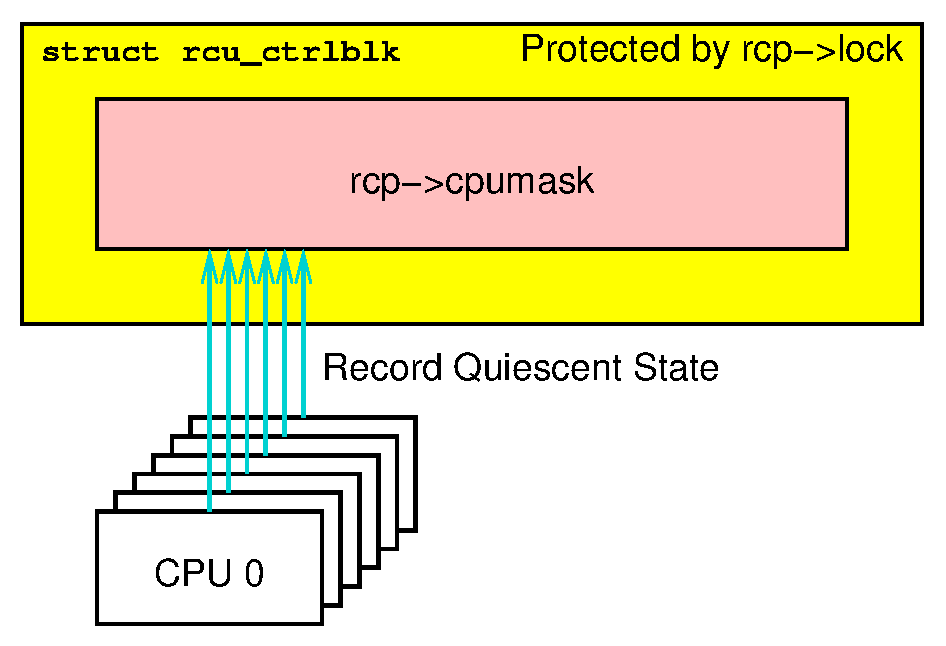
\includegraphics{appendix/rcuimpl/FlatClassicRCU}}
\end{center}
\caption{Flat Classic RCU State}
\label{fig:app:rcuimpl:rcutree:Flat Classic RCU State}
\end{figure}

Classic RCU's most important data structure is the \co{rcu_ctrlblk}
structure, which contains the \co{->cpumask} field, which contains
one bit per CPU, as shown in
Figure~\ref{fig:app:rcuimpl:rcutree:Flat Classic RCU State}.
Each CPU's bit is set to one at the beginning of each grace period,
and each CPU must clear its bit after it passes through a quiescent
state.
Because multiple CPUs might want to clear their bits concurrently,
which would corrupt the \co{->cpumask} field, a
\co{->lock}
spinlock is used to protect \co{->cpumask}, preventing any
such corruption.
Unfortunately, this spinlock can also suffer extreme contention if there
are more than a few hundred CPUs, which might soon become quite common
if multicore trends continue.
Worse yet, the fact that \emph{all} CPUs must clear their own bit means
that CPUs are not permitted to sleep through a grace period, which limits
Linux's ability to conserve power.




The next section lays out what we need from a new non-real-time
RCU implementation.

\subsection{RCU Desiderata}
\label{app:rcuimpl:rcutree:RCU Desiderata}

The list of real-time RCU desiderata~\cite{PaulMcKenney05b}
is a very good start:

\begin{enumerate}
\item	Deferred destruction, so that an RCU grace period cannot end
	until all pre-existing RCU read-side critical sections have
	completed.
\item	Reliable, so that RCU supports 24x7 operation for years at
	a time.
\item	Callable from irq handlers.
\item	Contained memory footprint, so that mechanisms exist to expedite
	grace periods if there are too many callbacks.  (This is weakened
	from the LCA2005 list.)
\item	Independent of memory blocks, so that RCU can work with any
	conceivable memory allocator.
\item	Synchronization-free read side, so that only normal non-atomic
	instructions operating on CPU- or task-local memory are permitted.
	(This is strengthened from the LCA2005 list.)
\item	Unconditional read-to-write upgrade, which is used in several
	places in the Linux kernel where the update-side lock is
	acquired within the RCU read-side critical section.
\item	Compatible API.

\item	Because this is not to be a real-time RCU, the requirement for
	preemptible RCU read-side critical sections can be dropped.
	However, we need to add the following new requirements to account
	for changes over the past few years.

\item	Scalability with extremely low internal-to-RCU lock contention.
	RCU must support at least 1,024 CPUs gracefully, and preferably
	at least 4,096.
\item	Energy conservation: RCU must be able to avoid awakening
	low-power-state dynticks-idle CPUs, but still determine
	when the current grace period ends.
	This has been implemented in real-time RCU, but needs serious
	simplification.
\item	RCU read-side critical sections must be permitted in NMI
	handlers as well as irq handlers.  Note that preemptible RCU
	was able to avoid this requirement due to a separately
	implemented \co{synchronize_sched()}.
\item	RCU must operate gracefully in face of repeated CPU-hotplug
	operations.
	This is simply carrying forward a requirement met by both
	classic and real-time.
\item	It must be possible to wait for all previously registered
	RCU callbacks to complete, though this is already provided
	in the form of \co{rcu_barrier()}.
\item	Detecting CPUs that are failing to respond is desirable,
	to assist diagnosis both of RCU and of various infinite
	loop bugs and hardware failures that can prevent RCU grace
	periods from ending.
\item	Extreme expediting of RCU grace periods is desirable,
	so that an RCU grace period can be forced to complete within
	a few hundred microseconds of the last relevant RCU read-side
	critical second completing.
	However, such an operation would be expected to incur
	severe CPU overhead, and would be primarily useful when
	carrying out a long sequence of operations that each needed
	to wait for an RCU grace period.
\end{enumerate}

The most pressing of the new requirements is the first one, scalability.
The next section therefore describes how to make order-of-magnitude reductions
in contention on RCU's internal locks.

\subsection{Towards a More Scalable RCU Implementation}
\label{app:rcuimpl:rcutree:Towards a More Scalable RCU Implementation}

\begin{figure}[htb]
\begin{center}
\resizebox{3in}{!}{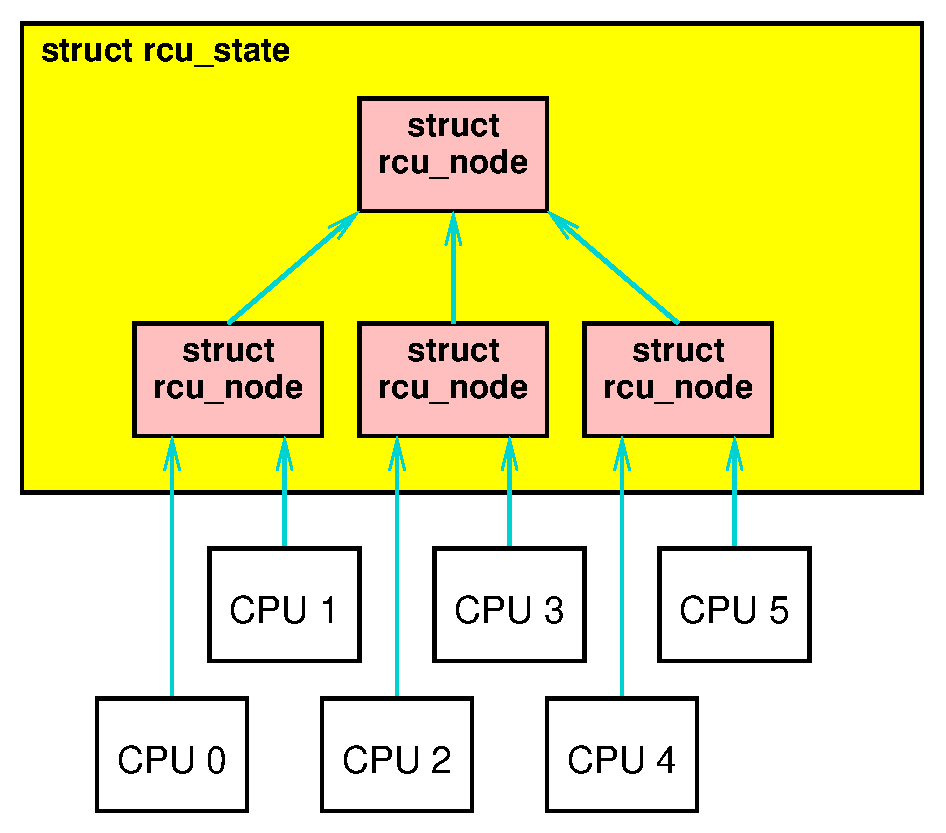
\includegraphics{appendix/rcuimpl/TreeClassicRCU}}
\end{center}
\caption{Hierarchical RCU State}
\label{fig:app:rcuimpl:rcutree:Hierarchical RCU State}
\end{figure}

One effective way to reduce lock contention is to create a hierarchy,
as shown in
Figure~\ref{fig:app:rcuimpl:rcutree:Hierarchical RCU State}.
Here, each of the four \co{rcu_node} structures has its own lock,
so that only CPUs~0 and 1 will acquire the lower left
\co{rcu_node}'s lock, only CPUs~2 and 3 will acquire the
lower middle \co{rcu_node}'s lock, and only CPUs~4 and 5
will acquire the lower right \co{rcu_node}'s lock.
During any given grace period,
only one of the CPUs accessing each of the lower \co{rcu_node}
structures will access the upper \co{rcu_node}, namely, the
last of each pair of CPUs to record a quiescent state for the corresponding
grace period.

This results in a significant reduction in lock contention:
instead of six CPUs contending for a single lock each grace period,
we have only three for the upper \co{rcu_node}'s lock
(a reduction of 50\%) and only
two for each of the lower \co{rcu_node}s' locks (a reduction
of 67\%).

\begin{figure}[htb]
\begin{center}
\resizebox{3in}{!}{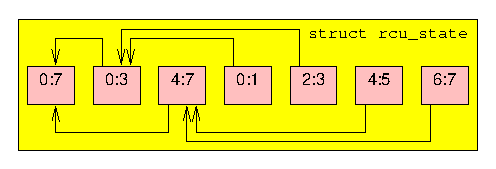
\includegraphics{appendix/rcuimpl/TreeMapping}}
\end{center}
\caption{Mapping {\tt rcu\_node} Hierarchy Into Array}
\label{fig:app:rcuimpl:rcutree:Mapping rcu-node Hierarchy Into Array}
\end{figure}

The tree of \co{rcu_node} structures is embedded into
a linear array in the \co{rcu_state} structure,
with the root of the tree in element zero, as shown in
Figure~\ref{fig:app:rcuimpl:rcutree:Mapping rcu-node Hierarchy Into Array}
for an eight-CPU
system with a three-level hierarchy.
Each arrow links a given \co{rcu_node} structure to its parent,
representing the \co{rcu_node}'s \co{->parent} field.
Each \co{rcu_node} indicates the range of CPUs covered,
so that the root node covers all of the CPUs, each node in the second
level covers half of the CPUs, and each node in the leaf level covering
a pair of CPUs.
This array is allocated statically at compile time based on the value
of \co{NR_CPUS}.

\begin{figure}[htbp]
\begin{center}
\resizebox{3in}{!}{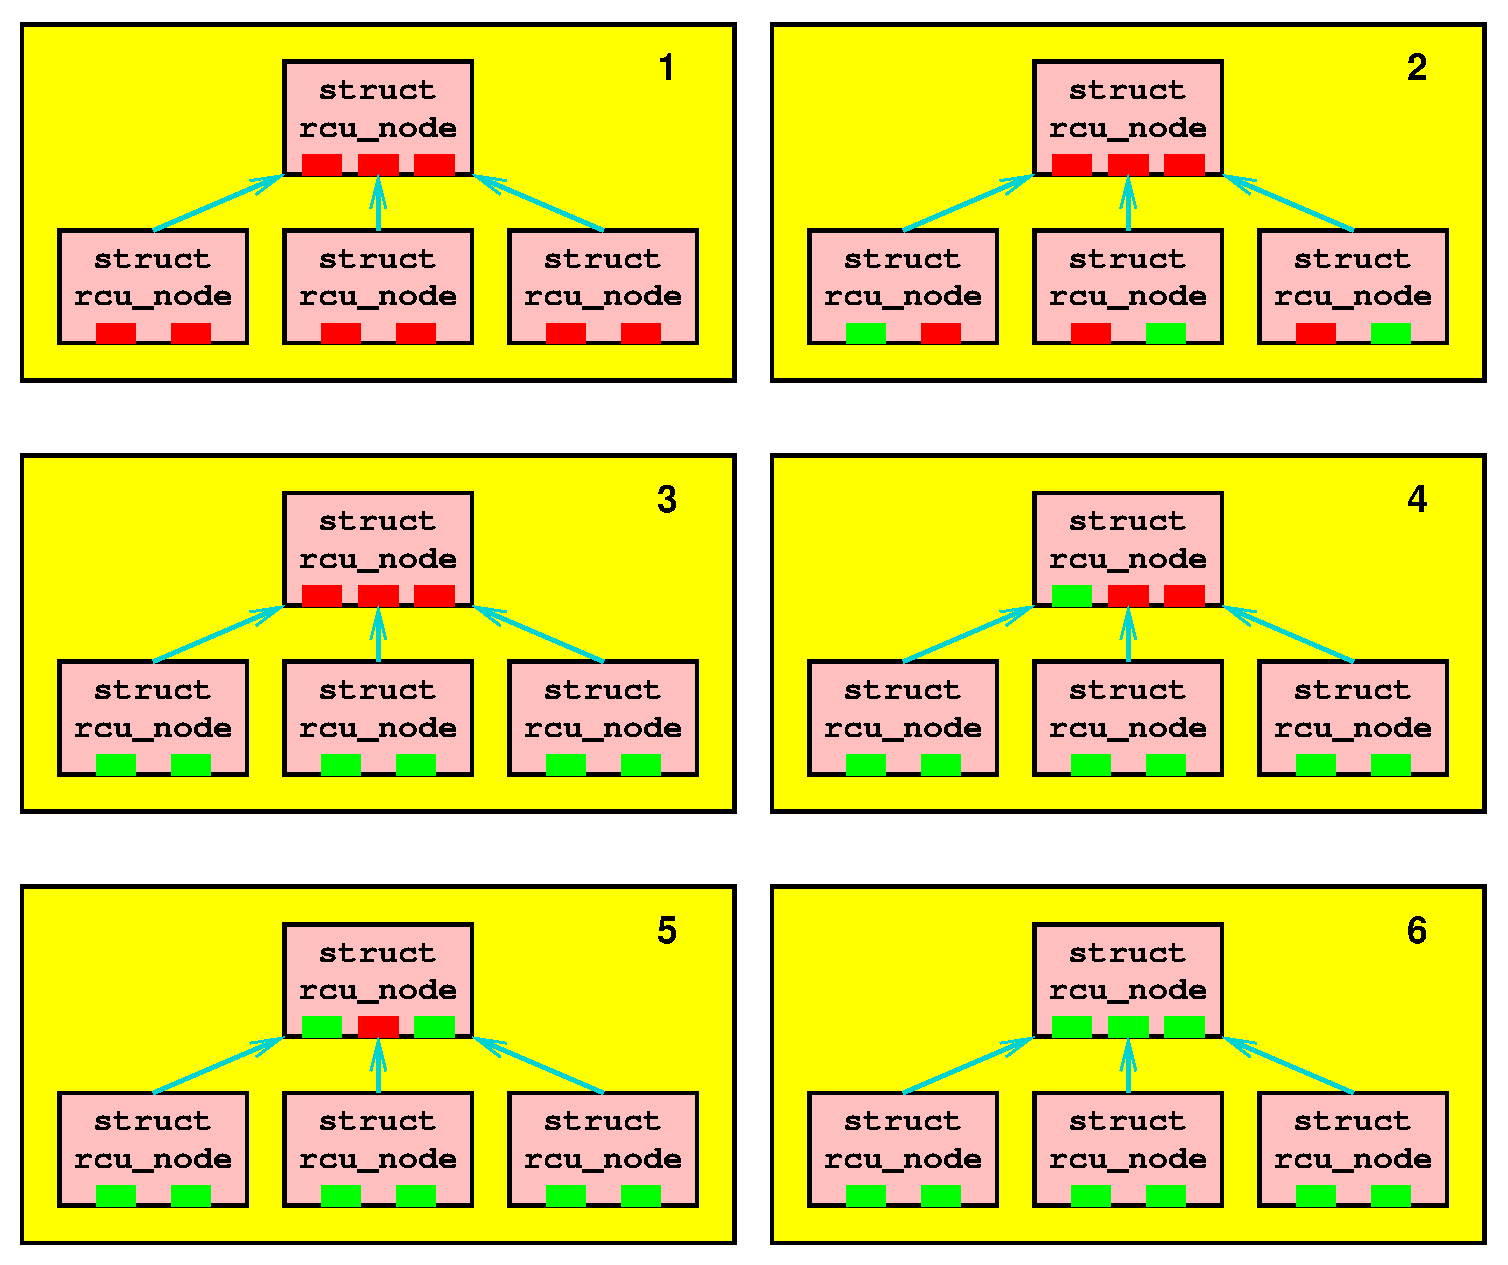
\includegraphics{appendix/rcuimpl/TreeClassicRCUGP}}
\end{center}
\caption{Hierarchical RCU Grace Period}
\label{fig:app:rcuimpl:rcutree:Hierarchical RCU Grace Period}
\end{figure}

The sequence of diagrams in
Figure~\ref{fig:app:rcuimpl:rcutree:Hierarchical RCU Grace Period}
shows how grace periods are detected.
In the first figure, no CPU has yet passed through a quiescent state,
as indicated by the red rectangles.
Suppose that all six CPUs simultaneously try to tell RCU that they have
passed through a quiescent state.
Only one of each pair will be able to acquire the lock on the
corresponding lower \co{rcu_node}, and so the second figure
shows the result if the lucky CPUs are numbers 0, 3, and 5, as indicated
by the green rectangles.
Once these lucky CPUs have finished, then the other CPUs will acquire
the lock, as shown in the third figure.
Each of these CPUs will see that they are the last in their group,
and therefore all three will attempt to move to the upper
\co{rcu_node}.
Only one at a time can acquire the upper \co{rcu_node} structure's
lock, and the fourth, fifth, and sixth figures show the sequence of
states assuming that CPU~1, CPU~2, and CPU~4 acquire
the lock in that order.
The sixth and final figure in the group shows that all CPUs have passed
through a quiescent state, so that the grace period has ended.

\begin{figure}[htb]
\begin{center}
\resizebox{3in}{!}{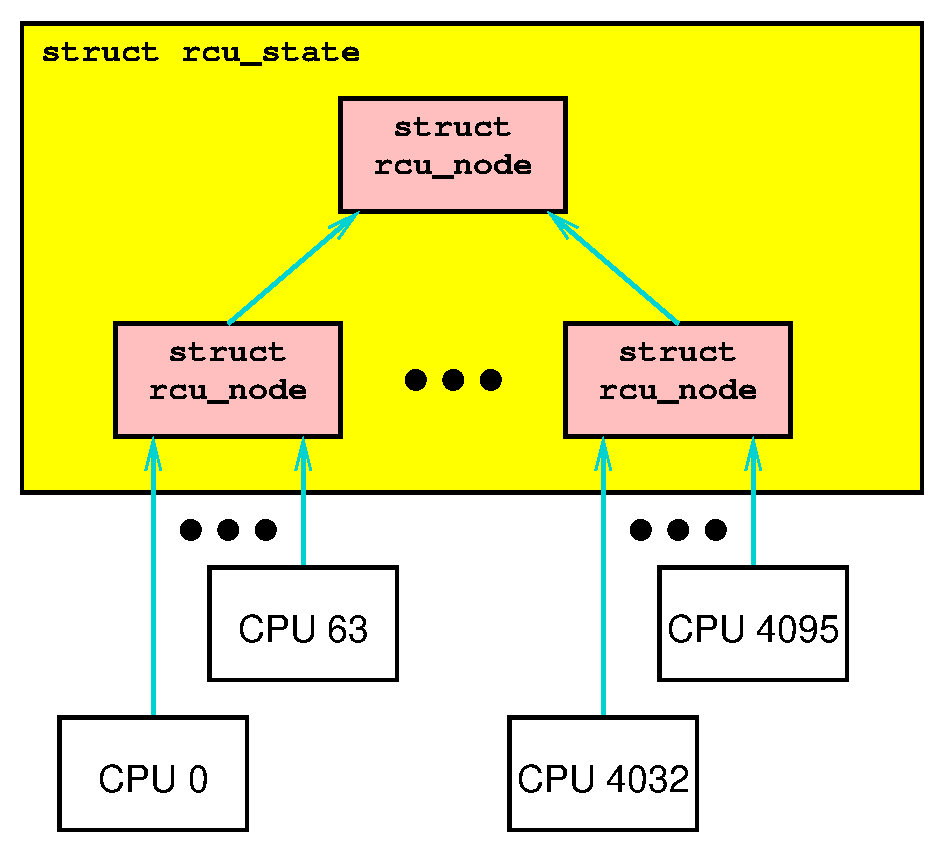
\includegraphics{appendix/rcuimpl/BigTreeClassicRCU}}
\end{center}
\caption{Hierarchical RCU State 4,096 CPUs}
\label{fig:app:rcuimpl:rcutree:Hierarchical RCU State 4,096 CPUs}
\end{figure}

In the above sequence, there were never more than three CPUs
contending for any one lock, in happy contrast to Classic RCU,
where all six CPUs might contend.
However, even more dramatic reductions in lock contention are
possible with larger numbers of CPUs.
Consider a hierarchy of \co{rcu_node} structures, with
64 lower structures and 64*64=4,096 CPUs, as shown in
Figure~\ref{fig:app:rcuimpl:rcutree:Hierarchical RCU State 4,096 CPUs}.

Here each of the lower \co{rcu_node} structures' locks
are acquired by 64 CPUs, a 64-times reduction from the 4,096 CPUs
that would acquire Classic RCU's single global lock.
Similarly, during a given grace period, only one CPU from each of
the lower \co{rcu_node} structures will acquire the
upper \co{rcu_node} structure's lock, which is again
a 64x reduction from the contention level that would be experienced
by Classic RCU running on a 4,096-CPU system.

\QuickQuiz{}
	Wait a minute!
	With all those new locks, how do you avoid deadlock?
\QuickQuizAnswer{
	Deadlock is avoided by never holding more than one of the
	\co{rcu_node} structures' locks at a given time.
	This algorithm uses two more locks, one to prevent CPU hotplug
	operations from running concurrently with grace-period advancement
	(\co{onofflock}) and another
	to permit only one CPU at a time from forcing a quiescent state
	to end quickly (\co{fqslock}).
	These are subject to a locking hierarchy, so that
	\co{fqslock} must be acquired before
	\co{onofflock}, which in turn must be acquired before
	any of the \co{rcu_node} structures' locks.

	Also, as a practical matter, refusing to ever hold more than
	one of the \co{rcu_node} locks means that it is unnecessary
	to track which ones are held.
	Such tracking would be painful as well as unnecessary.
} \QuickQuizEnd

\QuickQuiz{}
	Why stop at a 64-times reduction?
	Why not go for a few orders of magnitude instead?
\QuickQuizAnswer{
	RCU works with no problems on
	systems with a few hundred CPUs, so allowing 64 CPUs to contend on
	a single lock leaves plenty of headroom.
	Keep in mind that these locks are acquired quite rarely, as each
	CPU will check in about one time per grace period, and grace periods
	extend for milliseconds.
} \QuickQuizEnd

\QuickQuiz{}
	But I don't care about McKenney's lame excuses in the answer to
	Quick Quiz 2!!!
	I want to get the number of CPUs contending on a single lock down
	to something reasonable, like sixteen or so!!!
\QuickQuizAnswer{
	OK, have it your way, then!
	Set \co{CONFIG_RCU_FANOUT=16} and (for \co{NR_CPUS=4096})
	you will get a
	three-level hierarchy with with 256 \co{rcu_node} structures
	at the lowest level, 16 \co{rcu_node} structures as intermediate
	nodes, and a single root-level \co{rcu_node}.
	The penalty you will pay is that more \co{rcu_node} structures
	will need to be scanned when checking to see which CPUs need help
	completing their quiescent states (256 instead of only 64).
} \QuickQuizEnd

\begin{figure}[htb]
\begin{center}
\resizebox{3in}{!}{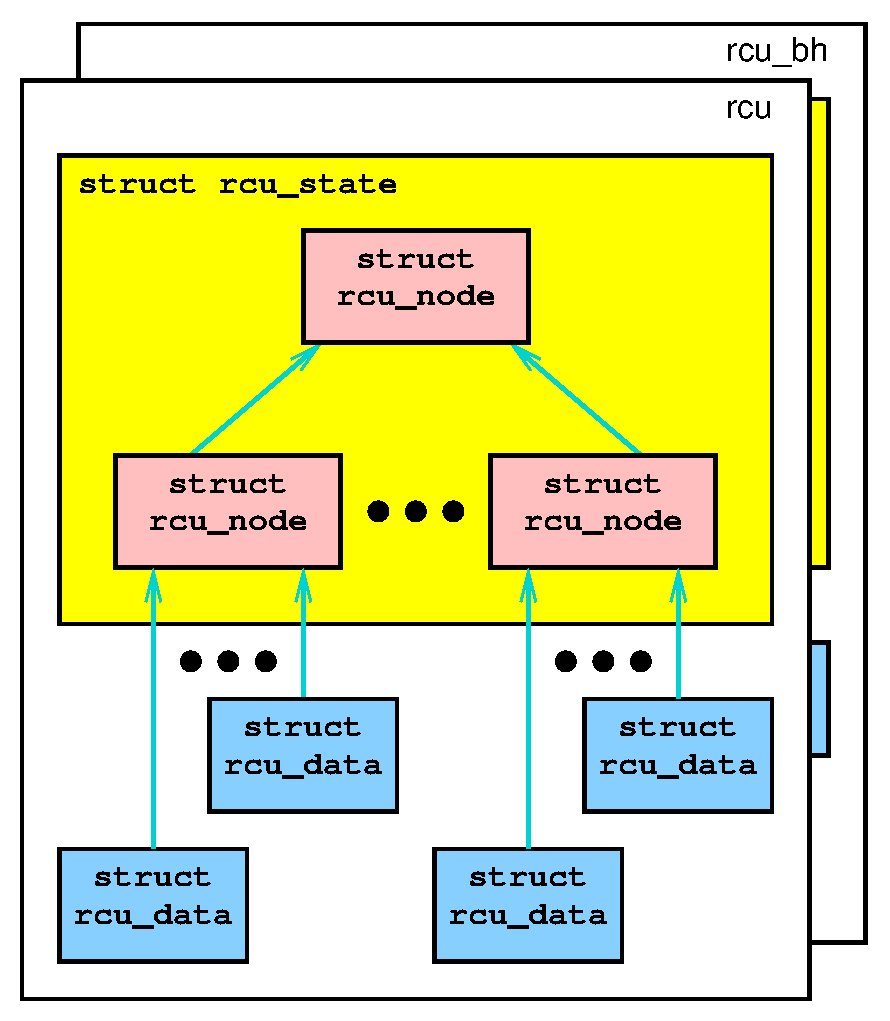
\includegraphics{appendix/rcuimpl/BigTreeClassicRCUBH}}
\end{center}
\caption{Hierarchical RCU State With BH}
\label{fig:app:rcuimpl:rcutree:Hierarchical RCU State With BH}
\end{figure}

The implementation maintains some per-CPU data, such as lists of
RCU callbacks, organized into \co{rcu_data} structures.
In addition, rcu (as in \co{call_rcu()}) and
rcu\_bh (as in \co{call_rcu_bh()}) each maintain their own
hierarchy, as shown in
Figure~\ref{fig:app:rcuimpl:rcutree:Hierarchical RCU State With BH}.

\QuickQuiz{}
	OK, so what is the story with the colors?
\QuickQuizAnswer{
	Data structures analogous to \co{rcu_state} (including
	\co{rcu_ctrlblk}) are yellow,
	those containing the bitmaps used to determine when CPUs have checked
	in are pink,
	and the per-CPU \co{rcu_data} structures are blue.
	The data structures used to conserve energy
	(such as \co{rcu_dynticks}) will be colored green.
} \QuickQuizEnd

The next section discusses energy conservation.

\subsection{Towards a Greener RCU Implementation}
\label{app:rcuimpl:rcutree:Towards a Greener RCU Implementation}

As noted earlier, an important goal of this effort is to leave sleeping
CPUs lie in order to promote energy conservation.
In contrast, classic RCU will happily awaken each and every sleeping CPU
at least once per grace period in some cases,
which is suboptimal in the case where
a small number of CPUs are busy doing RCU updates and the majority of
the CPUs are mostly idle.
This situation occurs frequently in systems sized for peak loads, and
we need to be able to accommodate it gracefully.
Furthermore, we need to fix a long-standing bug in Classic RCU where
a dynticks-idle CPU servicing an interrupt containing a long-running
RCU read-side critical section will fail to prevent an RCU grace period
from ending.

\QuickQuiz{}
	Given such an egregious bug, why does Linux run at all?
\QuickQuizAnswer{
	Because the Linux kernel contains device drivers that are (relatively)
	well behaved.
	Few if any of them spin in RCU read-side critical sections for the
	many milliseconds that would be required to provoke this bug.
	The bug nevertheless does need to be fixed, and this variant of
	RCU does fix it.
} \QuickQuizEnd

\begin{figure}[htb]
\begin{center}
\resizebox{3in}{!}{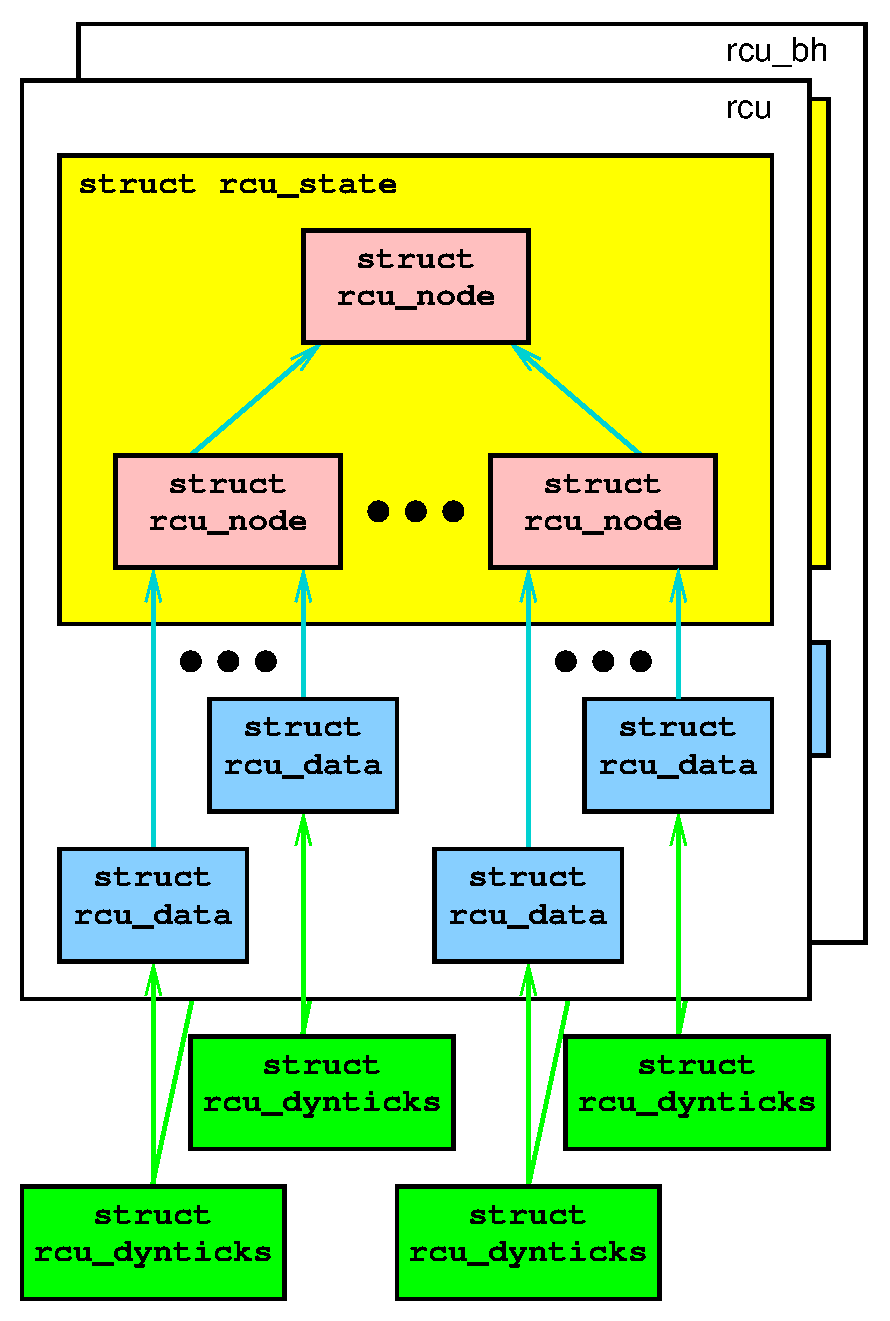
\includegraphics{appendix/rcuimpl/BigTreeClassicRCUBHdyntick}}
\end{center}
\caption{Hierarchical RCU State With Dynticks}
\label{fig:app:rcuimpl:rcutree:Hierarchical RCU State With Dynticks}
\end{figure}

This is accomplished by requiring that all CPUs manipulate counters
located in a per-CPU \co{rcu_dynticks} structure.
Loosely speaking, these counters have even-numbered values when the
corresponding CPU is in dynticks idle mode, and have odd-numbered values
otherwise.
RCU thus needs to wait for quiescent states only for those CPUs whose
\co{rcu_dynticks} counters are odd, and need not wake up sleeping
CPUs, whose counters will be even.
As shown in
Figure~\ref{fig:app:rcuimpl:rcutree:Hierarchical RCU State With Dynticks},
each per-CPU \co{rcu_dynticks} structure
is shared by the ``rcu'' and ``rcu\_bh'' implementations.

The following section presents a high-level view of the RCU state machine.

\subsection{State Machine}
\label{app:rcuimpl:rcutree:State Machine}

\begin{figure}[htbp]
\begin{center}
\resizebox{3in}{!}{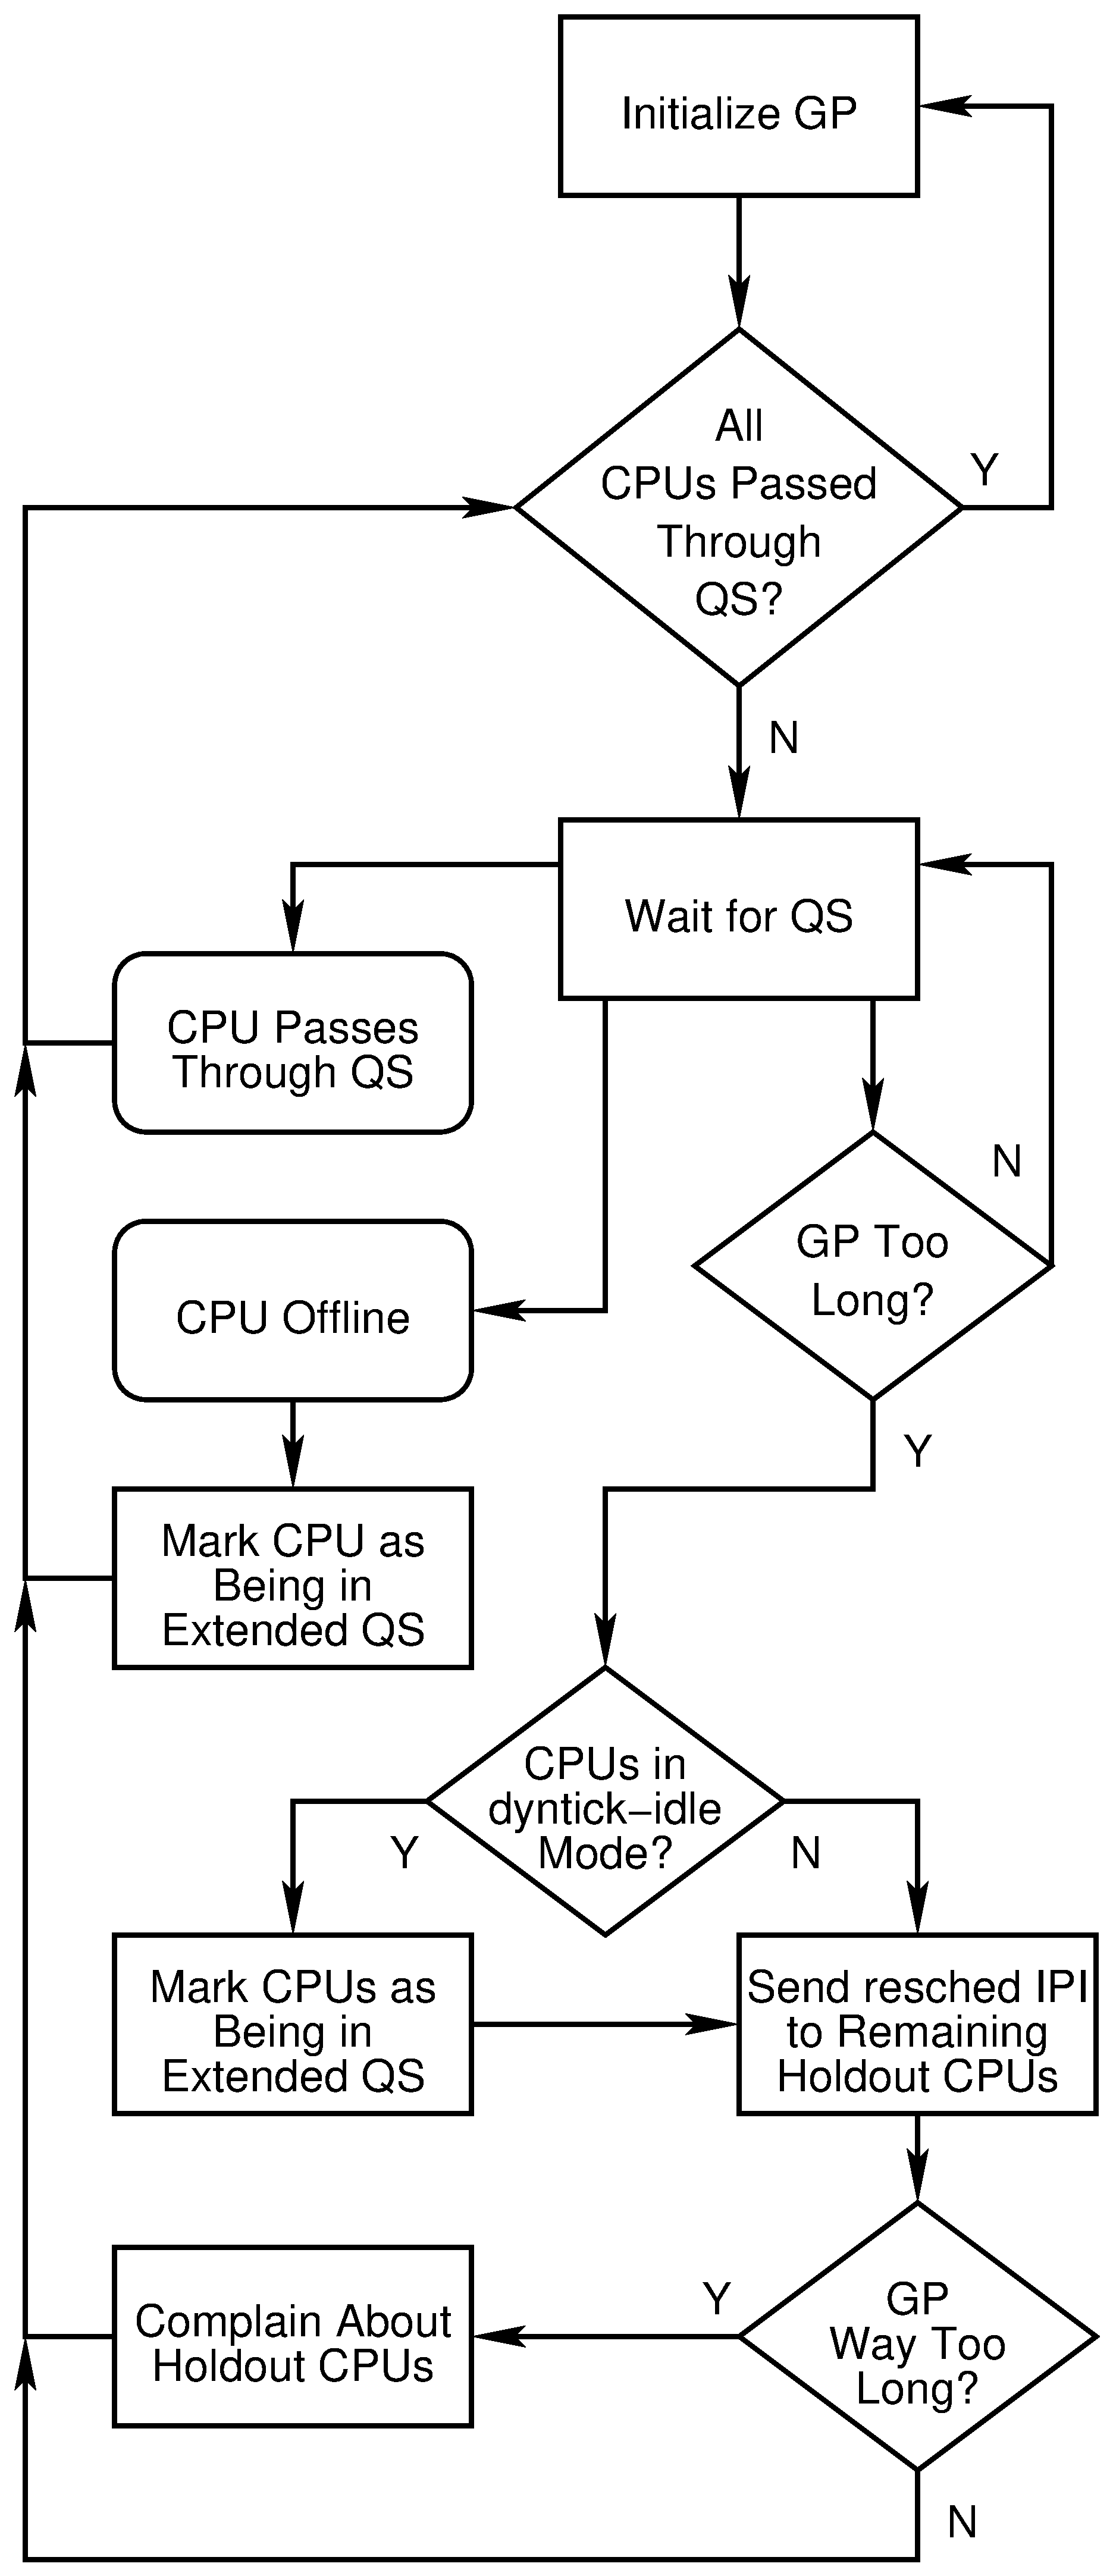
\includegraphics{appendix/rcuimpl/GenericRCUStateMachine}}
\end{center}
\caption{Generic RCU State Machine}
\label{fig:app:rcuimpl:rcutree:Generic RCU State Machine}
\end{figure}

At a sufficiently high level, Linux-kernel RCU implementations can
be thought of as high-level state machines as shown in
Figure~\ref{fig:app:rcuimpl:rcutree:Generic RCU State Machine}.
The common-case path through this state machine on a busy system
goes through the two uppermost loops, initializing at the
beginning of each grace period (GP),
waiting for quiescent states (QS), and noting when each CPU passes through
its first quiescent state for a given grace period.
On such a system, quiescent states will occur on each context switch,
or, for CPUs that are either idle or executing user-mode code, each
scheduling-clock interrupt.
CPU-hotplug events will take the state machine through the
``CPU Offline'' box, while the presence of ``holdout''
CPUs that fail to pass through quiescent states quickly enough will exercise
the path through the ``Send resched IPIs to Holdout CPUs'' box.
RCU implementations that avoid unnecessarily awakening dyntick-idle
CPUs will mark those CPUs as being in an extended quiescent state,
taking the ``Y'' branch out of the ``CPUs in dyntick-idle
Mode?'' decision diamond (but note that CPUs in dyntick-idle mode
will \emph{not} be sent resched IPIs).
Finally, if \co{CONFIG_RCU_CPU_STALL_DETECTOR} is enabled,
truly excessive delays in reaching quiescent states will exercise the
``Complain About Holdout CPUs'' path.

\QuickQuiz{}
	But doesn't this state diagram indicate that dyntick-idle CPUs will
	get hit with reschedule IPIs?  Won't that wake them up?
\QuickQuizAnswer{
	No.
	Keep in mind that RCU is handling groups of CPUs.
	One particular group might contain both dyntick-idle CPUs and
	CPUs in normal mode that have somehow managed to avoid passing through
	a quiescent state.
	Only the latter group will be sent a reschedule IPI; the dyntick-idle
	CPUs will merely be marked as being in an extended quiescent state.
} \QuickQuizEnd

\begin{figure}[htb]
\begin{center}
\resizebox{3in}{!}{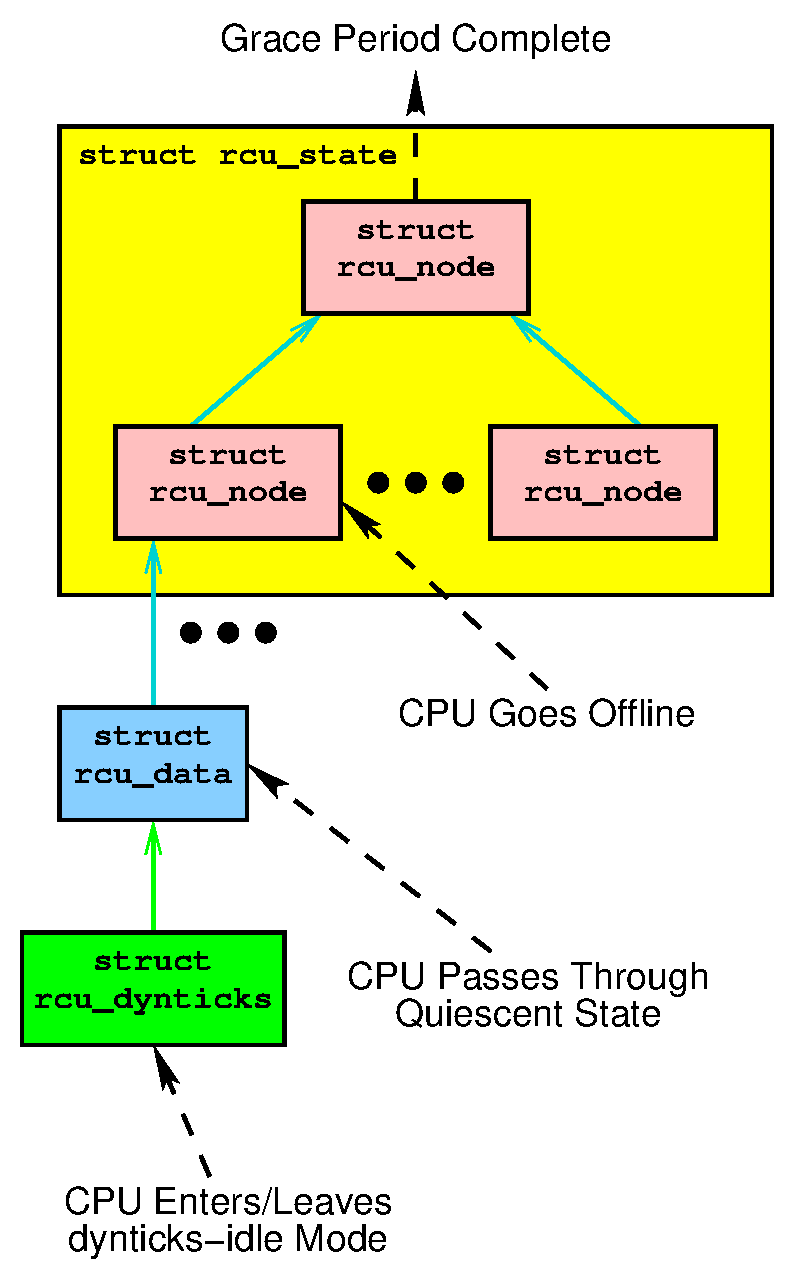
\includegraphics{appendix/rcuimpl/TreeRCUStateMachine}}
\end{center}
\caption{RCU State Machine and Hierarchical RCU Data Structures}
\label{fig:app:rcuimpl:rcutree:RCU State Machine and Hierarchical RCU Data Structures}
\end{figure}

The events in the above state schematic interact with different
data structures, as shown in
Figure~\ref{fig:app:rcuimpl:rcutree:RCU State Machine and Hierarchical RCU Data Structures}.
However, the state schematic does not directly translate into C code
for any of the RCU implementations.
Instead, these implementations are coded as an event-driven system within
the kernel.
Therefore, the following section describes some ``use cases'',
or ways in which the RCU algorithm traverses the above state schematic
as well as the relevant data structures.

\subsection{Use Cases}
\label{app:rcuimpl:rcutree:Use Cases}

This section gives an overview of several ``use cases''
within the RCU implementation, listing the data structures touched
and the functions invoked.
The use cases are as follows:

\begin{enumerate}
\item	Start a New Grace Period
	(Section~\ref{app:rcuimpl:rcutree:Start a New Grace Period})
\item	Pass Through a Quiescent State
	(Section~\ref{app:rcuimpl:rcutree:Pass Through a Quiescent State})
\item	Announce a Quiescent State to RCU
	(Section~\ref{app:rcuimpl:rcutree:Announce a Quiescent State to RCU})
\item	Enter and Leave Dynticks Idle Mode
	(Section~\ref{app:rcuimpl:rcutree:Enter and Leave Dynticks Idle Mode})
\item	Interrupt from Dynticks Idle Mode
	(Section~\ref{app:rcuimpl:rcutree:Interrupt from Dynticks Idle Mode})
\item	NMI from Dynticks Idle Mode
	(Section~\ref{app:rcuimpl:rcutree:NMI from Dynticks Idle Mode})
\item	Note That a CPU is in Dynticks Idle Mode
	(Section~\ref{app:rcuimpl:rcutree:Note That a CPU is in Dynticks Idle Mode})
\item	Offline a CPU
	(Section~\ref{app:rcuimpl:rcutree:Offline a CPU})
\item	Online a CPU
	(Section~\ref{app:rcuimpl:rcutree:Online a CPU})
\item	Detect a Too-Long Grace Period
	(Section~\ref{app:rcuimpl:rcutree:Detect a Too-Long Grace Period})
\end{enumerate}

Each of these use cases is described in the following sections.

\subsubsection{Start a New Grace Period}
\label{app:rcuimpl:rcutree:Start a New Grace Period}

The \co{rcu_start_gp()} function starts a new grace period.
This function is invoked when a CPU having callbacks waiting for a
grace period notices that no grace period is in progress.

The \co{rcu_start_gp()} function updates state in
the \co{rcu_state} and \co{rcu_data} structures
to note the newly started grace period,
acquires the \co{->onoff} lock (and disables irqs) to exclude
any concurrent CPU-hotplug operations,
sets the
bits in all of the \co{rcu_node} structures to indicate
that all CPUs (including this one) must pass through a quiescent
state,
and finally
releases the \co{->onoff} lock.

The bit-setting operation is carried out in two phases.
First, the non-leaf \co{rcu_node} structures' bits are set without
holding any additional locks, and then finally each leaf \co{rcu_node}
structure's bits are set in turn while holding that structure's
\co{->lock}.

\QuickQuiz{}
	But what happens if a CPU tries to report going through a quiescent
	state (by clearing its bit) before the bit-setting CPU has finished?
\QuickQuizAnswer{
	There are three cases to consider here:

	\begin{enumerate}
	\item	A CPU corresponding to a non-yet-initialized leaf
		\co{rcu_node} structure tries to report a quiescent state.
		This CPU will see its bit already cleared, so will give up on
		reporting its quiescent state.
		Some later quiescent state will serve for the new grace period.
	\item	A CPU corresponding to a leaf \co{rcu_node} structure that
		is currently being initialized tries to report a quiescent
		state.
		This CPU will see that the \co{rcu_node} structure's
		\co{->lock} is held, so will spin until it is
		released.
		But once the lock is released, the \co{rcu_node}
		structure will have been initialized, reducing to the
		following case.
	\item	A CPU corresponding to a leaf \co{rcu_node} that has
		already been initialized tries to report a quiescent state.
		This CPU will find its bit set, and will therefore clear it.
		If it is the last CPU for that leaf node, it will
		move up to the next level of the hierarchy.
		However, this CPU cannot possibly be the last CPU in the
		system to report a quiescent state, given that the CPU
		doing the initialization cannot yet have checked in.
	\end{enumerate}

	So, in all three cases, the potential race is resolved correctly.
} \QuickQuizEnd

\QuickQuiz{}
	And what happens if \emph{all} CPUs try to report going
	through a quiescent
	state before the bit-setting CPU has finished, thus ending the new
	grace period before it starts?
\QuickQuizAnswer{
	The bit-setting CPU cannot pass through a
	quiescent state during initialization, as it has irqs disabled.
	Its bits therefore remain non-zero, preventing the grace period from
	ending until the data structure has been fully initialized.
} \QuickQuizEnd

\subsubsection{Pass Through a Quiescent State}
\label{app:rcuimpl:rcutree:Pass Through a Quiescent State}

The rcu and rcu\_bh flavors of RCU have different sets of quiescent
states.
Quiescent states for rcu are context switch, idle (either dynticks or
the idle loop), and user-mode execution, while quiescent states for
rcu\_bh are any code outside of softirq with interrupts enabled.
Note that an quiescent state for rcu is also a quiescent state
for rcu\_bh.
Quiescent states for rcu are recorded by invoking \co{rcu_qsctr_inc()},
while quiescent states for rcu\_bh are recorded by invoking
\co{rcu_bh_qsctr_inc()}.
These two functions record their state in the current CPU's
\co{rcu_data} structure.

These functions are invoked from the scheduler, from
\co{__do_softirq()}, and from \co{rcu_check_callbacks()}.
This latter function is invoked from the scheduling-clock interrupt,
and analyzes state to determine whether this interrupt occurred within
a quiescent state, invoking \co{rcu_qsctr_inc()} and/or
\co{rcu_bh_qsctr_inc()}, as appropriate.
It also raises \co{RCU_SOFTIRQ}, which results in
\co{rcu_process_callbacks()} being invoked on the current
CPU at some later time from softirq context.

\subsubsection{Announce a Quiescent State to RCU}
\label{app:rcuimpl:rcutree:Announce a Quiescent State to RCU}

The afore-mentioned \co{rcu_process_callbacks()} function
has several duties:

\begin{enumerate}
\item	Determining when to take measures to end an over-long grace period
	(via \co{force_quiescent_state()}).
\item	Taking appropriate action when some other CPU detected the end of
	a grace period (via \co{rcu_process_gp_end()}).
	``Appropriate action`` includes advancing this CPU's
	callbacks and recording the new grace period.
	This same function updates state in response to some other
	CPU starting a new grace period.
\item	Reporting the current CPU's quiescent states to the core RCU
	mechanism (via \co{rcu_check_quiescent_state()}, which
	in turn invokes \co{cpu_quiet()}).
	This of course might mark the end of the current grace period.
\item	Starting a new grace period if there is no grace period in progress
	and this CPU has RCU callbacks still waiting for a grace period
	(via \co{cpu_needs_another_gp()} and
	\co{rcu_start_gp()}).
\item	Invoking any of this CPU's callbacks whose grace period has ended
	(via \co{rcu_do_batch()}).
\end{enumerate}

These interactions are carefully orchestrated in order to avoid
buggy behavior such as reporting a quiescent state from the previous
grace period against the current grace period.

\subsubsection{Enter and Leave Dynticks Idle Mode}
\label{app:rcuimpl:rcutree:Enter and Leave Dynticks Idle Mode}

The scheduler invokes \co{rcu_enter_nohz()} to
enter dynticks-idle mode, and invokes \co{rcu_exit_nohz()}
to exit it.
The \co{rcu_enter_nohz()} function increments a per-CPU
\co{dynticks_nesting} variable and
also a per-CPU \co{dynticks} counter, the latter of which which must
then have an even-numbered value.
The \co{rcu_exit_nohz()} function decrements this same
per-CPU \co{dynticks_nesting} variable,
and again increments the per-CPU \co{dynticks}
counter, the latter of which must then have an odd-numbered value.

The \co{dynticks} counter can be sampled by other CPUs.
If the value is even, the first CPU is in an extended quiescent state.
Similarly, if the counter value changes during a given grace period,
the first CPU must have been in an extended quiescent state at some
point during the grace period.
However, there is another \co{dynticks_nmi} per-CPU variable
that must also be sampled, as will be discussed below.

\subsubsection{Interrupt from Dynticks Idle Mode}
\label{app:rcuimpl:rcutree:Interrupt from Dynticks Idle Mode}

Interrupts from dynticks idle mode are handled by
\co{rcu_irq_enter()} and \co{rcu_irq_exit()}.
The \co{rcu_irq_enter()} function increments the
per-CPU \co{dynticks_nesting} variable, and, if the prior
value was zero, also increments the \co{dynticks}
per-CPU variable (which must then have an odd-numbered value).

The \co{rcu_irq_exit()} function decrements the
per-CPU \co{dynticks_nesting} variable, and, if the new
value is zero, also increments the \co{dynticks}
per-CPU variable (which must then have an even-numbered value).

Note that entering an irq handler exits dynticks idle mode
and vice versa.
This enter/exit anti-correspondence can cause much confusion.
You have been warned.

\subsubsection{NMI from Dynticks Idle Mode}
\label{app:rcuimpl:rcutree:NMI from Dynticks Idle Mode}

NMIs from dynticks idle mode are handled by \co{rcu_nmi_enter()}
and \co{rcu_nmi_exit()}.
These functions both increment the \co{dynticks_nmi} counter,
but only if the aforementioned \co{dynticks} counter is even.
In other words, NMI's refrain from manipulating the
\co{dynticks_nmi} counter if the NMI occurred in non-dynticks-idle
mode or within an interrupt handler.

The only difference between these two functions is the error checks,
as \co{rcu_nmi_enter()} must leave the \co{dynticks_nmi}
counter with an odd value, and \co{rcu_nmi_exit()} must leave
this counter with an even value.

\subsubsection{Note That a CPU is in Dynticks Idle Mode}
\label{app:rcuimpl:rcutree:Note That a CPU is in Dynticks Idle Mode}

The \co{force_quiescent_state()} function implements a
three-phase state machine.
The first phase (\co{RCU_INITIALIZING}) waits for \co{rcu_start_gp()}
to complete grace-period initialization.
This state is not exited by \co{force_quiescent_state()}, but rather
by \co{rcu_start_gp()}.

In the second phase (\co{RCU_SAVE_DYNTICK}), the
\co{dyntick_save_progress_counter()} function scans the CPUs that
have not yet reported a quiescent state, recording their per-CPU
\co{dynticks} and \co{dynticks_nmi} counters.
If these counters both have even-numbered values, then the corresponding
CPU is in dynticks-idle state, which is therefore noted as an extended
quiescent state (reported via \co{cpu_quiet_msk()}).

In the third phase (\co{RCU_FORCE_QS}), the
\co{rcu_implicit_dynticks_qs()} function again scans the CPUs
that have not yet reported a quiescent state (either explicitly or
implicitly during the \co{RCU_SAVE_DYNTICK} phase), again checking the
per-CPU \co{dynticks} and \co{dynticks_nmi} counters.
If each of these has either changed in value or is now even, then
the corresponding CPU has either passed through or is now in dynticks
idle, which as before is noted as an extended quiescent state.

If \co{rcu_implicit_dynticks_qs()} finds that a given CPU
has neither been in dynticks idle mode nor reported a quiescent state,
it invokes \co{rcu_implicit_offline_qs()}, which checks to see
if that CPU is offline, which is also reported as an extended quiescent
state.
If the CPU is online, then \co{rcu_implicit_offline_qs()} sends
it a reschedule IPI in an attempt to remind it of its duty to report
a quiescent state to RCU.

Note that \co{force_quiescent_state()} does not directly
invoke either \co{dyntick_save_progress_counter()} or
\co{rcu_implicit_dynticks_qs()}, instead passing these functions
to an intervening \co{rcu_process_dyntick()} function that
abstracts out the common code involved in scanning the CPUs and reporting
extended quiescent states.

\QuickQuiz{}
	And what happens if one CPU comes out of dyntick-idle mode and then
	passed through a quiescent state just as another CPU notices that the
	first CPU was in dyntick-idle mode?
	Couldn't they both attempt to report a quiescent state at the same
	time, resulting in confusion?
\QuickQuizAnswer{
	They will both attempt to acquire the lock on the same leaf
	\co{rcu_node} structure.
	The first one to acquire the lock will report the quiescent state
	and clear the appropriate bit, and the second one to acquire the
	lock will see that this bit has already been cleared.
} \QuickQuizEnd

\QuickQuiz{}
	But what if \emph{all} the CPUs end up in dyntick-idle mode?
	Wouldn't that prevent the current RCU grace period from ever ending?
\QuickQuizAnswer{
	Indeed it will!
	However, CPUs that have RCU callbacks are not permitted to enter
	dyntick-idle mode, so the only way that \emph{all} the CPUs could
	possibly end up in dyntick-idle mode would be if there were
	absolutely no RCU callbacks in the system.
	And if there are no RCU callbacks in the system, then there is no
	need for the RCU grace period to end.
	In fact, there is no need for the RCU grace period to even
	\emph{start}.

	RCU will restart if some irq handler does a \co{call_rcu()},
	which will cause an RCU callback to appear on the corresponding CPU,
	which will force that CPU out of dyntick-idle mode, which will in turn
	permit the current RCU grace period to come to an end.
} \QuickQuizEnd

\QuickQuiz{}
	Given that \co{force_quiescent_state()} is a three-phase state
	machine, don't we have triple the scheduling latency due to scanning
	all the CPUs?
\QuickQuizAnswer{
	Ah, but the three phases will not execute back-to-back on the same CPU,
	and, furthermore, the first (initialization) phase doesn't do any
	scanning.
	Therefore, the scheduling-latency hit of the three-phase algorithm
	is no different than that of a single-phase algorithm.
	If the scheduling latency becomes a problem, one approach would be to
	recode the state machine to scan the CPUs incrementally, most likely
	by keeping state on a per-leaf-\co{rcu_node} basis.
	But first show me a problem in the real world, \emph{then}
	I will consider fixing it!
} \QuickQuizEnd

\subsubsection{Offline a CPU}
\label{app:rcuimpl:rcutree:Offline a CPU}

CPU-offline events cause \co{rcu_cpu_notify()} to invoke
\co{rcu_offline_cpu()}, which in turn invokes
\co{__rcu_offline_cpu()} on both the rcu and the rcu\_bh
instances of the data structures.
This function clears the outgoing CPU's bits so that future grace
periods will not expect this CPU to announce quiescent states,
and further invokes \co{cpu_quiet()} in order to announce
the offline-induced extended quiescent state.
This work is performed with the global \co{->onofflock}
held in order to prevent interference with concurrent grace-period
initialization.

\QuickQuiz{}
	But the other reason to hold \co{->onofflock} is to prevent
	multiple concurrent online/offline operations, right?
\QuickQuizAnswer{
	Actually, no!
	The CPU-hotplug code's synchronization design prevents multiple
	concurrent CPU online/offline operations, so only one CPU
	online/offline operation can be executing at any given time.
	Therefore, the only purpose of \co{->onofflock} is to prevent a CPU
	online or offline operation from running concurrently with grace-period
	initialization.
} \QuickQuizEnd

\subsubsection{Online a CPU}
\label{app:rcuimpl:rcutree:Online a CPU}

CPU-online events cause \co{rcu_cpu_notify()} to invoke
\co{rcu_online_cpu()}, which initializes the incoming CPU's
dynticks state, and then invokes \co{rcu_init_percpu_data()}
to initialize the incoming CPU's \co{rcu_data} structure,
and also to set this CPU's bits (again protected by
the global \co{->onofflock}) so that future grace periods
will wait for a quiescent state from this CPU.
Finally, \co{rcu_online_cpu()}
sets up the RCU softirq vector for this CPU.

\QuickQuiz{}
	Given all these acquisitions of the global \co{->onofflock},
	won't there
	be horrible lock contention when running with thousands of CPUs?
\QuickQuizAnswer{
	Actually, there can be only three acquisitions of this lock per grace
	period, and each grace period lasts many milliseconds.
	One of the acquisitions is by the CPU initializing for the current
	grace period, and the other two onlining and offlining some CPU.
	These latter two cannot run concurrently due to the CPU-hotplug
	locking, so at most two CPUs can be contending for this lock at any
	given time.

	Lock contention on \co{->onofflock} should therefore
	be no problem, even on systems with thousands of CPUs.
} \QuickQuizEnd

\QuickQuiz{}
	Why not simplify the code by merging the detection of dyntick-idle
	CPUs with that of offline CPUs?
\QuickQuizAnswer{
	It might well be that such merging may eventually be the right
	thing to do.
	In the meantime, however, there are some challenges:

	\begin{enumerate}
	\item	CPUs are not allowed to go into dyntick-idle mode while they
		have RCU callbacks pending, but CPUs \emph{are} allowed to go
		offline with callbacks pending.
		This means that CPUs going offline need to have their callbacks
		migrated to some other CPU, thus, we cannot allow CPUs to
		simply go quietly offline.
	\item	Present-day Linux systems run with \co{NR_CPUS}
		much larger than the actual number of CPUs.
		A unified approach could thus end up uselessly waiting on
		CPUs that are not just offline, but which never existed in
		the first place.
	\item	RCU is already operational when CPUs get onlined one
		at a time during boot, and therefore must handle the online
		process.
		This onlining must exclude grace-period initialization, so
		the \co{->onofflock} must still be used.
	\item	CPUs often switch into and out of dyntick-idle mode
		extremely frequently, so it is not reasonable to use the
		heavyweight online/offline code path for entering and exiting
		dyntick-idle mode.
	\end{enumerate}
} \QuickQuizEnd

\subsubsection{Detect a Too-Long Grace Period}
\label{app:rcuimpl:rcutree:Detect a Too-Long Grace Period}

When the \co{CONFIG_RCU_CPU_STALL_DETECTOR} kernel parameter
is specified, the \co{record_gp_stall_check_time()} function
records the time and also a timestamp set three seconds into the future.
If the current grace period still has not ended by that time, the
\co{check_cpu_stall()} function will check for the culprit,
invoking \co{print_cpu_stall()} if the current CPU is the
holdout, or \co{print_other_cpu_stall()} if it is some other CPU.
A two-jiffies offset helps ensure that CPUs report on themselves
when possible, taking advantage of the fact that a CPU can normally
do a better job of tracing its own stack than it can tracing some other
CPU's stack.

\subsection{Testing}
\label{app:rcuimpl:rcutree:Testing}

RCU is fundamental synchronization code, so any failure of RCU
results in random, difficult-to-debug memory corruption.
It is therefore extremely important that RCU be \emph{highly} reliable.
Some of this reliability stems from careful design, but at the
end of the day we must also rely on heavy stress testing, otherwise
known as torture.

Fortunately, although there has been some debate as to exactly
what populations are covered by the provisions of the Geneva Convention
% <a href="http://www.unhchr.ch/html/menu3/b/91.htm">Geneva Convention</a>,
it is still the case that it does not apply to software.
Therefore, it is still legal to torture your software.
In fact, it is strongly encouraged, because if you don't torture your
software, it will end up torturing \emph{you} by crashing at the most
inconvenient times imaginable.

Therefore, we torture RCU quite vigorously using the rcutorture module.

However, it is not sufficient to torture the common-case uses of RCU.
It is also necessary to torture it in unusual situations, for example,
when concurrently onlining and offlining CPUs and when CPUs are concurrently
entering and exiting dynticks idle mode.
I use a script @@@ move to CodeSamples, ref @@@
% <a href="http://lwn.net/Articles/305786/">script</a> to online and offline CPUs,
and use the \co{test_no_idle_hz} module parameter to rcutorture
to stress-test dynticks idle mode.
Just to be fully paranoid, I sometimes run a kernbench workload in parallel
as well.
Ten hours of this sort of torture on a 128-way machine seems sufficient
to shake out most bugs.

Even this is not the complete story.
As Alexey Dobriyan and Nick Piggin demonstrated in early 2008, it is
also necessary to torture RCU with all relevant combinations of kernel
parameters.
The relevant kernel parameters may be identified using yet another
script @@@ move to CodeSamples, ref @@@
% <a href="http://lwn.net/Articles/305787/">script</a>, and are as follows:

\begin{enumerate}
\item    \co{CONFIG_CLASSIC_RCU}: Classic RCU.
\item    \co{CONFIG_PREEMPT_RCU}: Preemptible (real-time) RCU.
\item    \co{CONFIG_TREE_RCU}: Classic RCU for huge SMP systems.
\item    \co{CONFIG_RCU_FANOUT}: Number of children for each
		\co{rcu_node}.
\item    \co{CONFIG_RCU_FANOUT_EXACT}: Balance the
		\co{rcu_node} tree.
\item    \co{CONFIG_HOTPLUG_CPU}: Allow CPUs to be offlined
		and onlined.
\item    \co{CONFIG_NO_HZ}: Enable dyntick-idle mode.
\item    \co{CONFIG_SMP}: Enable multi-CPU operation.
\item    \co{CONFIG_RCU_CPU_STALL_DETECTOR}: Enable RCU to detect
		when CPUs go on extended quiescent-state vacations.
\item    \co{CONFIG_RCU_TRACE}: Generate RCU trace files in debugfs.
\end{enumerate}

We ignore the \co{CONFIG_DEBUG_LOCK_ALLOC} configuration
variable under the perhaps-naive assumption that hierarchical RCU
could not have broken lockdep.
There are still 10 configuration variables, which would result in
1,024 combinations if they were independent boolean variables.
Fortunately the first three are mutually exclusive, which reduces
the number of combinations down to 384, but \co{CONFIG_RCU_FANOUT}
can take on values from 2 to 64, increasing the number of combinations
to 12,096.
This is an infeasible number of combinations.

One key observation is that only \co{CONFIG_NO_HZ}
and \co{CONFIG_PREEMPT} can be expected to have changed behavior
if either \co{CONFIG_CLASSIC_RCU} or
\co{CONFIG_PREEMPT_RCU} are in effect, as only these portions
of the two pre-existing RCU implementations were changed during this effort.
This cuts out almost two thirds of the possible combinations.

Furthermore, not all of the possible values of
\co{CONFIG_RCU_FANOUT} produce significantly different results,
in fact only a few cases really need to be tested separately:

\begin{enumerate}
\item	Single-node ``tree''.
\item	Two-level balanced tree.
\item	Three-level balanced tree.
\item	Autobalanced tree, where \co{CONFIG_RCU_FANOUT}
	specifies an unbalanced tree, but such that it is auto-balanced
	in absence of \co{CONFIG_RCU_FANOUT_EXACT}.
\item	Unbalanced tree.
\end{enumerate}

Looking further, \co{CONFIG_HOTPLUG_CPU} makes sense only
given \co{CONFIG_SMP}, and \co{CONFIG_RCU_CPU_STALL_DETECTOR}
is independent, and really only needs to be tested once (though someone
even more paranoid than am I might decide to test it both with
and without \co{CONFIG_SMP}).
Similarly, \co{CONFIG_RCU_TRACE} need only be tested once,
but the truly paranoid (such as myself) will choose to run it both with
and without \co{CONFIG_NO_HZ}.

This allows us to obtain excellent coverage of RCU with only 15
test cases.
All test cases specify the following configuration parameters in order
to run rcutorture and so that \co{CONFIG_HOTPLUG_CPU=n} actually
takes effect:

\vspace{5pt}
\begin{minipage}[t]{\columnwidth}
\small
\begin{verbatim}
CONFIG_RCU_TORTURE_TEST=m
CONFIG_MODULE_UNLOAD=y
CONFIG_SUSPEND=n
CONFIG_HIBERNATION=n
\end{verbatim}
\end{minipage}
\vspace{5pt}

The 15 test cases are as follows:

\begin{enumerate}
\item	Force single-node ``tree'' for small systems:

\vspace{5pt}
\begin{minipage}[t]{\columnwidth}
\small
\begin{verbatim}
	CONFIG_NR_CPUS=8
	CONFIG_RCU_FANOUT=8
	CONFIG_RCU_FANOUT_EXACT=n
	CONFIG_RCU_TRACE=y
	CONFIG_PREEMPT_RCU=n
	CONFIG_CLASSIC_RCU=n
	CONFIG_TREE_RCU=y
\end{verbatim}
\end{minipage}
\vspace{5pt}

\item	Force two-level tree for large systems:

\vspace{5pt}
\begin{minipage}[t]{\columnwidth}
\small
\begin{verbatim}
	CONFIG_NR_CPUS=8
	CONFIG_RCU_FANOUT=4
	CONFIG_RCU_FANOUT_EXACT=n
	CONFIG_RCU_TRACE=n
	CONFIG_PREEMPT_RCU=n
	CONFIG_CLASSIC_RCU=n
	CONFIG_TREE_RCU=y
\end{verbatim}
\end{minipage}
\vspace{5pt}

\item	Force three-level tree for huge systems:

\vspace{5pt}
\begin{minipage}[t]{\columnwidth}
\small
\begin{verbatim}
	CONFIG_NR_CPUS=8
	CONFIG_RCU_FANOUT=2
	CONFIG_RCU_FANOUT_EXACT=n
	CONFIG_RCU_TRACE=y
	CONFIG_PREEMPT_RCU=n
	CONFIG_CLASSIC_RCU=n
	CONFIG_TREE_RCU=y
\end{verbatim}
\end{minipage}
\vspace{5pt}

\item	Test autobalancing to a balanced tree:

\vspace{5pt}
\begin{minipage}[t]{\columnwidth}
\small
\begin{verbatim}
	CONFIG_NR_CPUS=8
	CONFIG_RCU_FANOUT=6
	CONFIG_RCU_FANOUT_EXACT=n
	CONFIG_RCU_TRACE=y
	CONFIG_PREEMPT_RCU=n
	CONFIG_CLASSIC_RCU=n
	CONFIG_TREE_RCU=y
\end{verbatim}
\end{minipage}
\vspace{5pt}

\item	Test unbalanced tree:

\vspace{5pt}
\begin{minipage}[t]{\columnwidth}
\small
\begin{verbatim}
	CONFIG_NR_CPUS=8
	CONFIG_RCU_FANOUT=6
	CONFIG_RCU_FANOUT_EXACT=y
	CONFIG_RCU_CPU_STALL_DETECTOR=y
	CONFIG_RCU_TRACE=y
	CONFIG_PREEMPT_RCU=n
	CONFIG_CLASSIC_RCU=n
	CONFIG_TREE_RCU=y
\end{verbatim}
\end{minipage}
\vspace{5pt}

\item	Disable CPU-stall detection:

\vspace{5pt}
\begin{minipage}[t]{\columnwidth}
\small
\begin{verbatim}
	CONFIG_SMP=y
	CONFIG_NO_HZ=y
	CONFIG_RCU_CPU_STALL_DETECTOR=n
	CONFIG_HOTPLUG_CPU=y
	CONFIG_RCU_TRACE=y
	CONFIG_PREEMPT_RCU=n
	CONFIG_CLASSIC_RCU=n
	CONFIG_TREE_RCU=y
\end{verbatim}
\end{minipage}
\vspace{5pt}

\item	Disable CPU-stall detection and dyntick idle mode:

\vspace{5pt}
\begin{minipage}[t]{\columnwidth}
\small
\begin{verbatim}
	CONFIG_SMP=y
	CONFIG_NO_HZ=n
	CONFIG_RCU_CPU_STALL_DETECTOR=n
	CONFIG_HOTPLUG_CPU=y
	CONFIG_RCU_TRACE=y
	CONFIG_PREEMPT_RCU=n
	CONFIG_CLASSIC_RCU=n
	CONFIG_TREE_RCU=y
\end{verbatim}
\end{minipage}
\vspace{5pt}

\item	Disable CPU-stall detection and CPU hotplug:

\vspace{5pt}
\begin{minipage}[t]{\columnwidth}
\small
\begin{verbatim}
	CONFIG_SMP=y
	CONFIG_NO_HZ=y
	CONFIG_RCU_CPU_STALL_DETECTOR=n
	CONFIG_HOTPLUG_CPU=n
	CONFIG_RCU_TRACE=y
	CONFIG_PREEMPT_RCU=n
	CONFIG_CLASSIC_RCU=n
	CONFIG_TREE_RCU=y
\end{verbatim}
\end{minipage}
\vspace{5pt}

\item	Disable CPU-stall detection, dyntick idle mode, and CPU hotplug:

\vspace{5pt}
\begin{minipage}[t]{\columnwidth}
\small
\begin{verbatim}
	CONFIG_SMP=y
	CONFIG_NO_HZ=n
	CONFIG_RCU_CPU_STALL_DETECTOR=n
	CONFIG_HOTPLUG_CPU=n
	CONFIG_RCU_TRACE=y
	CONFIG_PREEMPT_RCU=n
	CONFIG_CLASSIC_RCU=n
	CONFIG_TREE_RCU=y
\end{verbatim}
\end{minipage}
\vspace{5pt}

\item	Disable SMP, CPU-stall detection, dyntick idle mode, and CPU hotplug:

\vspace{5pt}
\begin{minipage}[t]{\columnwidth}
\small
\begin{verbatim}
	CONFIG_SMP=n
	CONFIG_NO_HZ=n
	CONFIG_RCU_CPU_STALL_DETECTOR=n
	CONFIG_HOTPLUG_CPU=n
	CONFIG_RCU_TRACE=y
	CONFIG_PREEMPT_RCU=n
	CONFIG_CLASSIC_RCU=n
	CONFIG_TREE_RCU=y
\end{verbatim}
\end{minipage}
\vspace{5pt}
	This combination located a number of compiler warnings.

\item	Disable SMP and CPU hotplug:

\vspace{5pt}
\begin{minipage}[t]{\columnwidth}
\small
\begin{verbatim}
	CONFIG_SMP=n
	CONFIG_NO_HZ=y
	CONFIG_RCU_CPU_STALL_DETECTOR=y
	CONFIG_HOTPLUG_CPU=n
	CONFIG_RCU_TRACE=y
	CONFIG_PREEMPT_RCU=n
	CONFIG_CLASSIC_RCU=n
	CONFIG_TREE_RCU=y
\end{verbatim}
\end{minipage}
\vspace{5pt}

\item	Test Classic RCU with dynticks idle but without preemption:

\vspace{5pt}
\begin{minipage}[t]{\columnwidth}
\small
\begin{verbatim}
	CONFIG_NO_HZ=y
	CONFIG_PREEMPT=n
	CONFIG_RCU_TRACE=y
	CONFIG_PREEMPT_RCU=n
	CONFIG_CLASSIC_RCU=y
	CONFIG_TREE_RCU=n
\end{verbatim}
\end{minipage}
\vspace{5pt}

\item	Test Classic RCU with preemption but without dynticks idle:

\vspace{5pt}
\begin{minipage}[t]{\columnwidth}
\small
\begin{verbatim}
	CONFIG_NO_HZ=n
	CONFIG_PREEMPT=y
	CONFIG_RCU_TRACE=y
	CONFIG_PREEMPT_RCU=n
	CONFIG_CLASSIC_RCU=y
	CONFIG_TREE_RCU=n
\end{verbatim}
\end{minipage}
\vspace{5pt}

\item	Test Preemptible RCU with dynticks idle:

\vspace{5pt}
\begin{minipage}[t]{\columnwidth}
\small
\begin{verbatim}
	CONFIG_NO_HZ=y
	CONFIG_PREEMPT=y
	CONFIG_RCU_TRACE=y
	CONFIG_PREEMPT_RCU=y
	CONFIG_CLASSIC_RCU=n
	CONFIG_TREE_RCU=n
\end{verbatim}
\end{minipage}
\vspace{5pt}
\item	Test Preemptible RCU without dynticks idle:

\vspace{5pt}

\begin{minipage}[t]{\columnwidth}
\small
\begin{verbatim}
	CONFIG_NO_HZ=n
	CONFIG_PREEMPT=y
	CONFIG_RCU_TRACE=y
	CONFIG_PREEMPT_RCU=y
	CONFIG_CLASSIC_RCU=n
	CONFIG_TREE_RCU=n
\end{verbatim}
\end{minipage}
\vspace{5pt}
\end{enumerate}

For a large change that affects RCU core code, one should run
rcutorture for each of the above combinations, and concurrently
with CPU offlining and onlining for cases with
\co{CONFIG_HOTPLUG_CPU}.
For small changes, it may suffice to run kernbench in each case.
Of course, if the change is confined to a particular subset of
the configuration parameters, it may be possible to reduce the
number of test cases.

Torturing software: the Geneva Convention does not (yet) prohibit
it, and I strongly recommend it!

\subsection{Conclusion}
\label{app:rcuimpl:rcutree:Conclusion}

This hierarchical implementation of RCU reduces lock contention,
avoids unnecessarily awakening dyntick-idle sleeping CPUs, while
helping to debug Linux's hotplug-CPU code paths.
This implementation is designed to handle single systems with
thousands of CPUs, and on 64-bit systems has an architectural
limitation of a quarter million CPUs, a limit I expect to be
sufficient for at least the next few years.

This RCU implementation of course has some limitations:

\begin{enumerate}
\item	The \co{force_quiescent_state()} can scan the full
	set of CPUs with irqs disabled.
	This would be fatal in a real-time implementation of RCU,
	so if hierarchy ever needs to be introduced to preemptible
	RCU, some other approach will be required.
	It is possible that it will be problematic on 4,096-CPU
	systems, but actual testing on such systems is required
	to prove this one way or the other.
	
	On busy systems, the \co{force_quiescent_state()} scan
	would not be expected to happen,
	as CPUs should pass through quiescent states within three
	jiffies of the start of a quiescent state.  On semi-busy
	systems, only the CPUs in dynticks-idle mode throughout would
	need to be scanned.
	In some cases, for example when a dynticks-idle CPU is handling
	an interrupt during a scan, subsequent scans are required.
	However, each such scan is performed separately, so scheduling
	latency is degraded by the overhead of only one such scan.
	
	If this scan proves problematic, one straightforward solution
	would be to do the scan incrementally.
	This would increase code complexity slightly and would also
	increase the time required to end a grace period, but would
	nonetheless be a likely solution.
	
\item	The \co{rcu_node} hierarchy is created at compile
	time, and is therefore sized for the worst-case \co{NR_CPUS}
	number of CPUs.
	However, even for 4,096 CPUs, the \co{rcu_node}
	hierarchy consumes only 65 cache lines on a 64-bit machine
	(and just you try accommodating 4,096 CPUs on a 32-bit machine!).
	Of course, a kernel built with \co{NR_CPUS=4096}
	running on a 16-CPU machine would use a two-level tree when
	a single-node tree would work just fine.
	Although this configuration would incur added locking overhead,
	this does not affect hot-path read-side code, so should not be a
	problem in practice.
	
\item	This patch does increase kernel text and data somewhat:
	the old Classic RCU implementation consumes 1,757 bytes of
	kernel text and 456 bytes of kernel data for a total of 2,213 bytes,
	while the new hierarchical RCU implementation consumes 4,006
	bytes of kernel text and 624 bytes of kernel data for a total
	of 4,630 bytes on a \co{NR_CPUS=4} system.
	This is a non-problem even for most embedded systems, which
	often come with hundreds of megabytes of main memory.
	However, if this is a problem for tiny embedded systems, it may
	be necessary to provide both ``scale up'' and
	``scale down'' implementations of RCU.
\end{enumerate}

This hierarchical RCU implementation should nevertheless be a vast
improvement over Classic RCU for machines with hundreds of CPUs.
After all, Classic RCU was designed for systems with only 16-32 CPUs.

At some point, it may be necessary to also apply hierarchy to the
preemptible RCU implementation.
This will be challenging due to the modular arithmetic used on the
per-CPU counter pairs, but should be doable.
